The given equation can be expressed as 
\begin{align} \labl{5/11/Eq b}
\myvec{1 & 2}\vec{x} =-3 
\end{align}
Let 
\begin{align}
\vec{x}=\myvec{p\\0}
\end{align}
Substituting in equation \eqref{5/11/Eq b},
\begin{align}
\myvec{1 & 2} \myvec{p\\0} &= -3
\\ \implies p&= -3
\end{align}
Similarly, for 
\begin{align}
\vec{x}=\myvec{0\\q},
\end{align}
substituting in equation \eqref{5/11/Eq b},
\begin{align}
\myvec{1 & 2} \myvec{0\\q} &= -3
\\ \implies q &= \frac{-3}{2}
\end{align}
So, the intercepts of X and Y axes can be obtained as,
\begin{align}
\vec{A}=\myvec{-3\\0} , 
\vec{B}=\myvec{0\\\dfrac{-3}{2}}
\end{align}
%
See Fig. \ref{5/11/Fig:1}.
%
\begin{figure}[h]
\centering
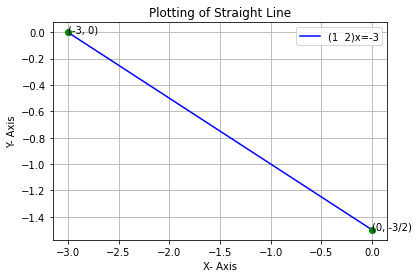
\includegraphics[width=\columnwidth]{solutions/5/11/graph.png}
\caption{Plot obtained from Python code}
\label{5/11/Fig:1}
\end{figure}


